\documentclass{article}
\usepackage[dvipsnames]{xcolor}
\usepackage[paperwidth=9cm, paperheight=5cm, margin = 0cm, top=0.5cm]{geometry}
\usepackage{amsmath}


\usepackage{pgf}
\usepackage{tikz}
\usetikzlibrary{positioning, calc}
\usetikzlibrary{arrows,automata}

\tikzstyle{source}  = 
[
	draw,circle,fill=black,thick,inner sep=0mm,minimum size=2mm
]

\tikzstyle{box}  =
[
	draw,rectangle,thick,inner sep=2mm,
	minimum width=8mm, minimum height=8mm
]

\tikzstyle{redbox} = 
[
	draw,rectangle,thick,inner sep=2mm,
	minimum width=8mm, minimum height=8mm,
	fill=red, opacity=0.3, text opacity=1, draw opacity=1
]

\tikzstyle{dredbox} = 
[
	draw,rectangle,thick,inner sep=2mm,
	minimum width=8mm, minimum height=8mm,
	fill=red, opacity=0.5, text opacity=1, draw opacity=1
]


\tikzstyle{bluebox} = 
[
	draw,rectangle,thick,inner sep=2mm,
	minimum width=8mm, minimum height=8mm,
	fill=blue, opacity=0.3, text opacity=1, draw opacity=1
]

\tikzstyle{greenbox} = 
[
	draw,rectangle,thick,inner sep=2mm,
	minimum width=8mm, minimum height=8mm,
	fill=green, opacity=0.3, text opacity=1, draw opacity=1
]

\tikzstyle{lgreenbox} = 
[
	draw,rectangle,thick,inner sep=2mm,
	minimum width=8mm, minimum height=8mm,
	fill=SpringGreen
]

\tikzstyle{dgreenbox} = 
[
	draw,rectangle,thick,inner sep=2mm,
	minimum width=8mm, minimum height=8mm,
	fill=ForestGreen, opacity=0.5, text opacity=1, draw opacity=1
]


\tikzstyle{bluestate}  = 
[
	state, draw=blue, line width=2pt,
	fill=LimeGreen
]

\tikzstyle{redstate}  = 
[
	state, draw=red, line width=2pt,
	fill=LimeGreen
]

\tikzstyle{violetstate}  = 
[
	state, draw=Violet, line width=2pt,
	fill=LimeGreen
]



\renewcommand{\vec}[1]{\boldsymbol{#1}}

\begin{document}
\begin{center}
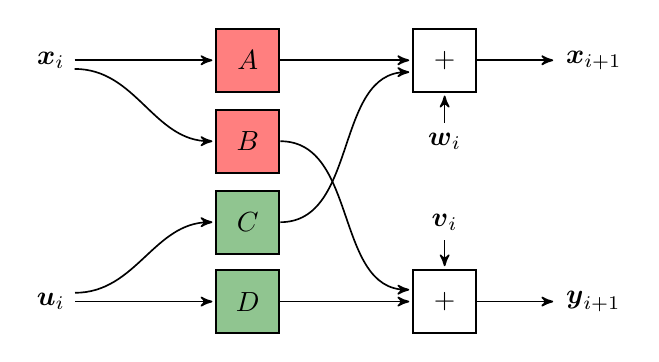
\begin{tikzpicture}[->,>=stealth',shorten >=1pt,auto,node distance=2.5cm,semithick]
         
\node(X1) {$\vec{x}_i$};
\node(U1) [below=2.6cm of X1] {$\vec{u}_i$};
\node[dredbox](X2) [right of=X1]{$A$};
\node[dredbox](W2)[below=0.2cm of X2] {$B$};
\node[dgreenbox](V2)[below=0.2cm of W2] {$C$};
\node[dgreenbox](U2) [right of=U1]{$D$};
\node[box](X3) [right of=X2]{$+$};
\node[box](U3) [right of=U2]{$+$};
\node(W3) [right of=W2]{$\vec{w}_i$};
\node(V3) [right of=V2]{$\vec{v}_i$};

\node(X4) [right = 1cm of X3]{$\vec{x}_{i+1}$};
\node(U4) [right = 1cm of U3]{$\vec{y}_{i+1}$};

\path
    (X1) edge (X2) 
	(X2) edge (X3)
	(X3) edge (X4)
	(X1.340) edge[in=180, out=0] (W2.180) 
	(W2.0)   edge[in=180, out=0] (U3.160);

\path
    (U1) edge (U2) 
	(U2) edge (U3)
	(U3) edge (U4)
    (U1.20) edge [in=180, out=0] (V2.180) 
	(V2.0)   edge[in=180, out=0] (X3.200);

\path
    (W3) edge (X3) 
    (V3) edge (U3); 
                   

\end{tikzpicture}
\end{center}

\end{document}
